\documentclass[12pt,a4paper]{article}
\usepackage[T1]{fontenc}
\usepackage[spanish]{babel}
\usepackage{amsmath, amssymb}
\usepackage{graphicx}
\usepackage{float}
\usepackage{booktabs}
\usepackage{xcolor}
\usepackage{listings}
\usepackage{hyperref}
\usepackage{geometry}
\geometry{margin=2.5cm}
\lstset{inputencoding=utf8, extendedchars=true}
\lstset{
  literate=
    {á}{{\'a}}1 {é}{{\'e}}1 {í}{{\'i}}1 {ó}{{\'o}}1 {ú}{{\'u}}1
    {Á}{{\'A}}1 {É}{{\'E}}1 {Í}{{\'I}}1 {Ó}{{\'O}}1 {Ú}{{\'U}}1
    {ñ}{{\~n}}1 {Ñ}{{\~N}}1
}
\definecolor{codegreen}{rgb}{0,0.6,0}
\definecolor{codegray}{rgb}{0.5,0.5,0.5}
\definecolor{codepurple}{rgb}{0.58,0,0.82}
\definecolor{backcolour}{rgb}{0.95,0.95,0.95}

\lstdefinelanguage{bash}{
  morekeywords={sudo,apt,cd,ls,echo,pip,python},
  sensitive=true,
  morecomment=[l]{\#},
  morestring=[b]"
}

\lstdefinestyle{mystyle}{
    backgroundcolor=\color{backcolour},   
    commentstyle=\color{codegreen},
    keywordstyle=\color{codepurple},
    numberstyle=\tiny\color{codegray},
    stringstyle=\color{codegreen},
    basicstyle=\ttfamily\footnotesize,
    breakatwhitespace=false,         
    breaklines=true,                 
    captionpos=b,                    
    keepspaces=true,                 
    numbers=left,                    
    numbersep=5pt,                  
    showspaces=false,                
    showstringspaces=false,
    showtabs=false,                  
    tabsize=2
}

\lstset{style=mystyle}

\title{\Large{\textbf{Simulación de Eventos Discretos: Análisis de una Peluquería}}}
\author{Mauro Eduardo Campver Barrios C-311}
\date{\today}

\begin{document}

\maketitle

\begin{abstract}
Este estudio presenta el análisis de un sistema de peluquería mediante simulación de eventos discretos. Se modeló la peluquería $"m@ripuri"$ como un sistema con llegadas aleatorias de clientes siguiendo una distribución de Poisson, tiempos de servicio exponenciales y capacidad limitada. Se analizaron indicadores de rendimiento como tiempos de espera, longitud de colas y probabilidad de rechazo. Además, se incluyó un análisis de sensibilidad para evaluar el impacto de contratar personal adicional. Los resultados demuestran que la contratación de una ayudante reduciría significativamente los tiempos de espera y la probabilidad de rechazo, mejorando sustancialmente la calidad del servicio.
\end{abstract}

\section{Introducción}

\subsection{Descripción del proyecto}
Se desarrolló una simulación de eventos discretos para analizar el desempeño de la peluquería "m@ripuri", la cual atiende a los clientes según el principio de "primero en entrar, primero en salir" (FIFO). La simulación modela la llegada de clientes con un proceso de Poisson (media de 5 clientes/hora) y tiempos de atención exponencialmente distribuidos (tiempo medio de 10 minutos por cliente). Además, se consideró la capacidad limitada del local: 1 sillón de atención y 4 sillas de espera.

\subsection{Objetivos y metas}

\begin{itemize}
    \item Estimar el número medio de clientes en el sistema y en la cola.
    \item Calcular la probabilidad de rechazo (cuando llega un cliente y no hay sitio disponible).
    \item Determinar el tiempo medio de espera y la probabilidad de que un cliente espere más de 45 minutos.
    \item Realizar un análisis de sensibilidad para evaluar el impacto de contratar una ayudante, lo que reduciría el tiempo de servicio a 5 minutos por cliente.
\end{itemize}

\subsection{Variables que describen el problema}

\begin{itemize}
    \item Tasa de llegada ($\lambda$): 5 clientes/hora.
    \item Tasa de servicio ($\mu$): 6 clientes/hora (equivalente a 10 minutos/cliente en el escenario actual).
    \item Capacidad máxima del sistema: 5 clientes (1 atendido + 4 en espera).
    \item Tiempo de espera en cola y en el sistema.
    \item Utilización del servidor y probabilidad de rechazo.
\end{itemize}

\section{Detalles de Implementación}

\subsection{Metodología}
La implementación de la simulación siguió un enfoque basado en eventos discretos, donde cada evento representa un cambio en el estado del sistema. Los principales pasos seguidos fueron:

\begin{enumerate}
    \item \textbf{Modelado del sistema}: Se definieron los eventos básicos (llegadas y salidas) y se implementó la lógica de la simulación utilizando una cola de eventos (heap) y una cola para los clientes.
    
    \item \textbf{Generación de tiempos}: Se usaron distribuciones exponenciales para modelar tanto los tiempos interllegada como los tiempos de servicio.
    
    \item \textbf{Mecanismo de rechazo}: Se implementó la lógica para rechazar clientes cuando el sistema alcanzaba su capacidad máxima (5 clientes en total).
    
    \item \textbf{Recopilación de estadísticas}: Durante la simulación se almacenaron variables como el número de clientes en el sistema, tiempos de espera, tiempos de servicio, utilización del servidor y la probabilidad de que los clientes esperen más de 45 minutos.
    
    \item \textbf{Validación}: Se realizó un análisis de parada de la simulación, ejecutándola en distintos periodos (desde 50 hasta 5000 horas) para verificar la convergencia de los resultados.
    
    \item \textbf{Modelo analítico}: Se implementó además un modelo teórico M/M/1/K que permitió comparar las métricas teóricas con los resultados simulados.
    
    \item \textbf{Análisis de sensibilidad}: Se evaluó el efecto de contratar una ayudante (reduciendo el tiempo de atención a 5 minutos) y se compararon las métricas de desempeño para ambos escenarios.
\end{enumerate}

\subsection{Implementación en Python}
La simulación se implementó utilizando Python con las bibliotecas NumPy, Matplotlib, Pandas, Seaborn y SciPy. Se utilizó una estructura orientada a objetos para encapsular la lógica del modelo de simulación.

\section{Resultados y Experimentos}

\subsection{Resultados de la simulación}

Los resultados de la simulación con un periodo de 4000 horas (incluyendo 100 horas de calentamiento) se presentan a continuación:

\begin{lstlisting}[language=bash, caption=Resultados de la simulación]
===== RESULTADOS DE LA SIMULACIÓN =====
Tiempo total de simulación: 4000 horas (con 100 horas de calentamiento)
Tasa de llegada: 5.0 clientes/hora
Tasa de servicio: 6.0 clientes/hora
Capacidad máxima: 5 clientes

--- Estadísticas ---
Clientes totales que llegaron: 20135
Clientes atendidos: 18076
Clientes rechazados: 2059
Probabilidad de rechazo: 0.1023

Número medio de clientes en el salón: 2.1278
Número medio de clientes esperando: 1.2410
Tiempo medio de espera: 16.45 minutos
Tiempo medio en el sistema: 26.47 minutos
Utilización del servidor: 88.68%
Probabilidad de esperar más de 45 minutos: 0.1150
\end{lstlisting}

\subsection{Comparación con el modelo teórico}

Se implementó un modelo teórico M/M/1/K para comparar con los resultados de la simulación:

\begin{lstlisting}[language=bash, caption=Comparación entre modelo teórico y simulación]
===== COMPARACIÓN MODELO TEÓRICO VS SIMULACIÓN =====
Modelo teórico M/M/1/5
Utilización teórica del servidor: 0.8333
Utilización simulada del servidor: 0.8814
Número medio teórico de clientes en el sistema: 1.9788
Número medio simulado de clientes en el sistema: 2.1120
Número medio teórico de clientes en cola: 1.0795
Número medio simulado de clientes en cola: 1.2306
Probabilidad teórica de sistema lleno: 0.1007
Probabilidad simulada de rechazo: 0.1059
Probabilidad teórica de esperar > 45 min: 0.4248
Probabilidad simulada de esperar > 45 min: 0.1196
\end{lstlisting}

\subsection{Análisis de sensibilidad}

Se realizó un análisis de sensibilidad para evaluar el impacto de diferentes tiempos de servicio, simulando el escenario de contratación de una ayudante:

\begin{lstlisting}[language=bash, caption=Análisis de sensibilidad]
===== ANÁLISIS DE SENSIBILIDAD: EFECTO DE CONTRATAR UNA AYUDANTE =====
Comparación de diferentes tiempos medios de servicio:
   service_time_min  sim_avg_system_length  sim_avg_queue_length  sim_rejection_probability  sim_prob_wait_over_45min
0              10.0               2.053705              1.176774                   0.101739                  0.110535
1               7.5               1.537515              0.692363                   0.043452                  0.031381
2               6.0               1.271633              0.439617                   0.013903                  0.006817
3               5.0               1.073262              0.248514                   0.006446                  0.001346
\end{lstlisting}

\subsection{Gráficos de la simulación}

Los resultados gráficos de la simulación proporcionan una visualización clara del comportamiento del sistema a lo largo del tiempo y bajo diferentes condiciones.

\begin{figure}[H]
    \centering
    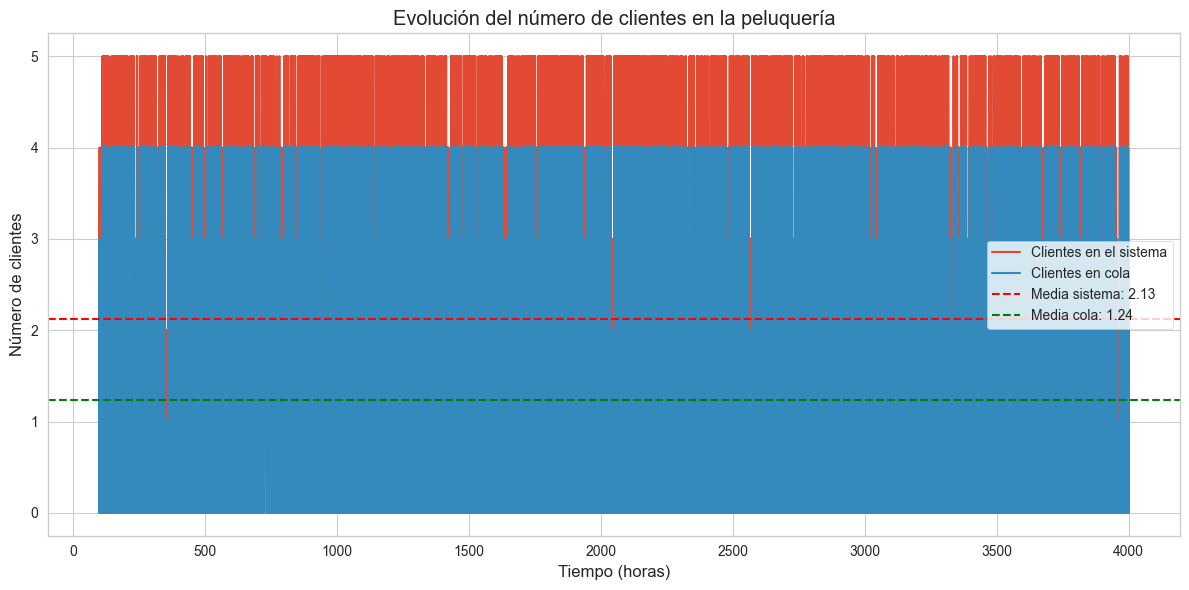
\includegraphics[width=0.8\textwidth]{clientes_sistema_tiempo.png}
    \caption{Evolución del número de clientes en la peluquería a lo largo del tiempo. La línea azul muestra los clientes en cola, mientras que la línea naranja representa los clientes totales en el sistema.}
    \label{fig:clientes_sistema}
\end{figure}

\begin{figure}[H]
    \centering
    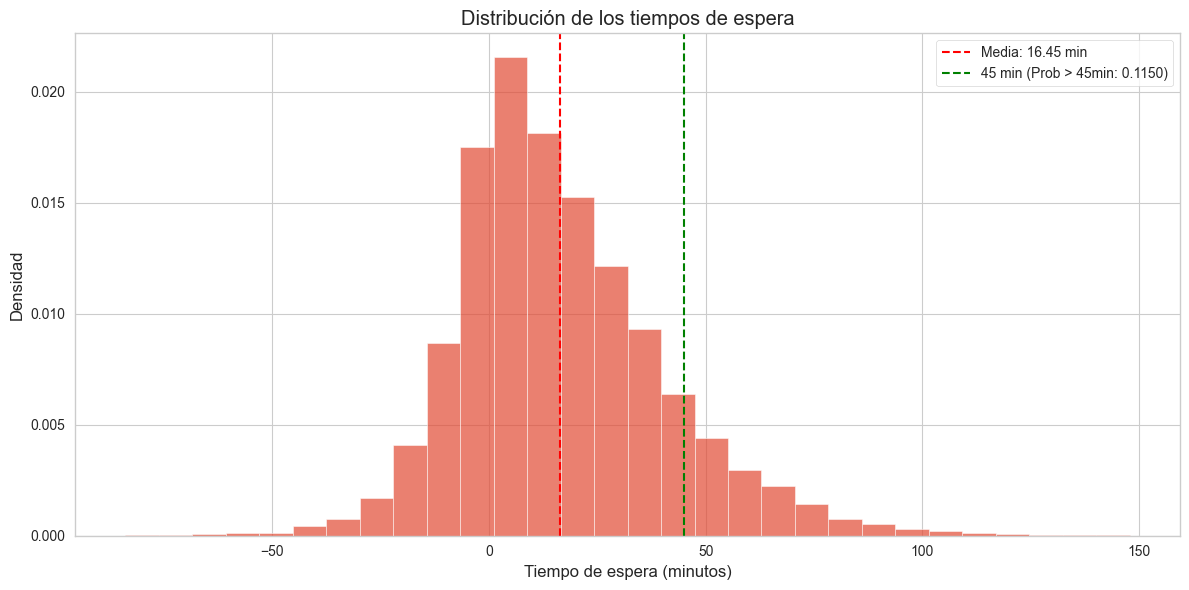
\includegraphics[width=0.8\textwidth]{distribucion_tiempos_espera.png}
    \caption{Distribución de los tiempos de espera en minutos. La línea roja vertical indica el tiempo medio de espera, mientras que la línea verde marca el umbral de 45 minutos.}
    \label{fig:tiempos_espera}
\end{figure}

\begin{figure}[H]
    \centering
    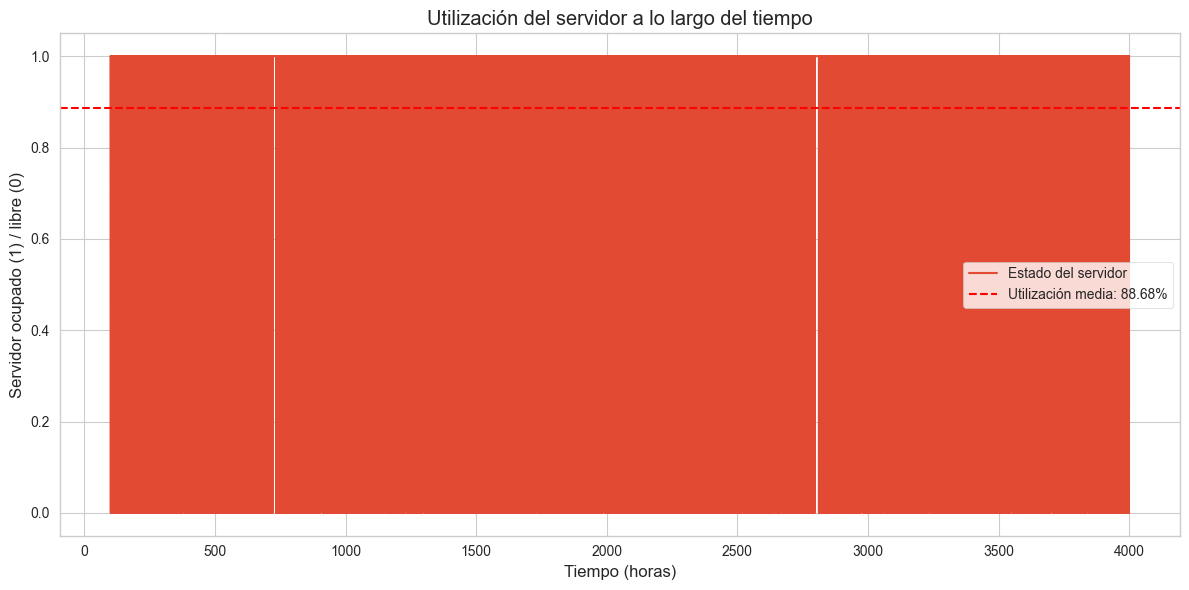
\includegraphics[width=0.8\textwidth]{utilizacion_servidor.png}
    \caption{Utilización del servidor a lo largo del tiempo. Los valores 1 indican que el servidor está ocupado, mientras que 0 indica que está libre.}
    \label{fig:utilizacion_servidor}
\end{figure}

\begin{figure}[H]
    \centering
    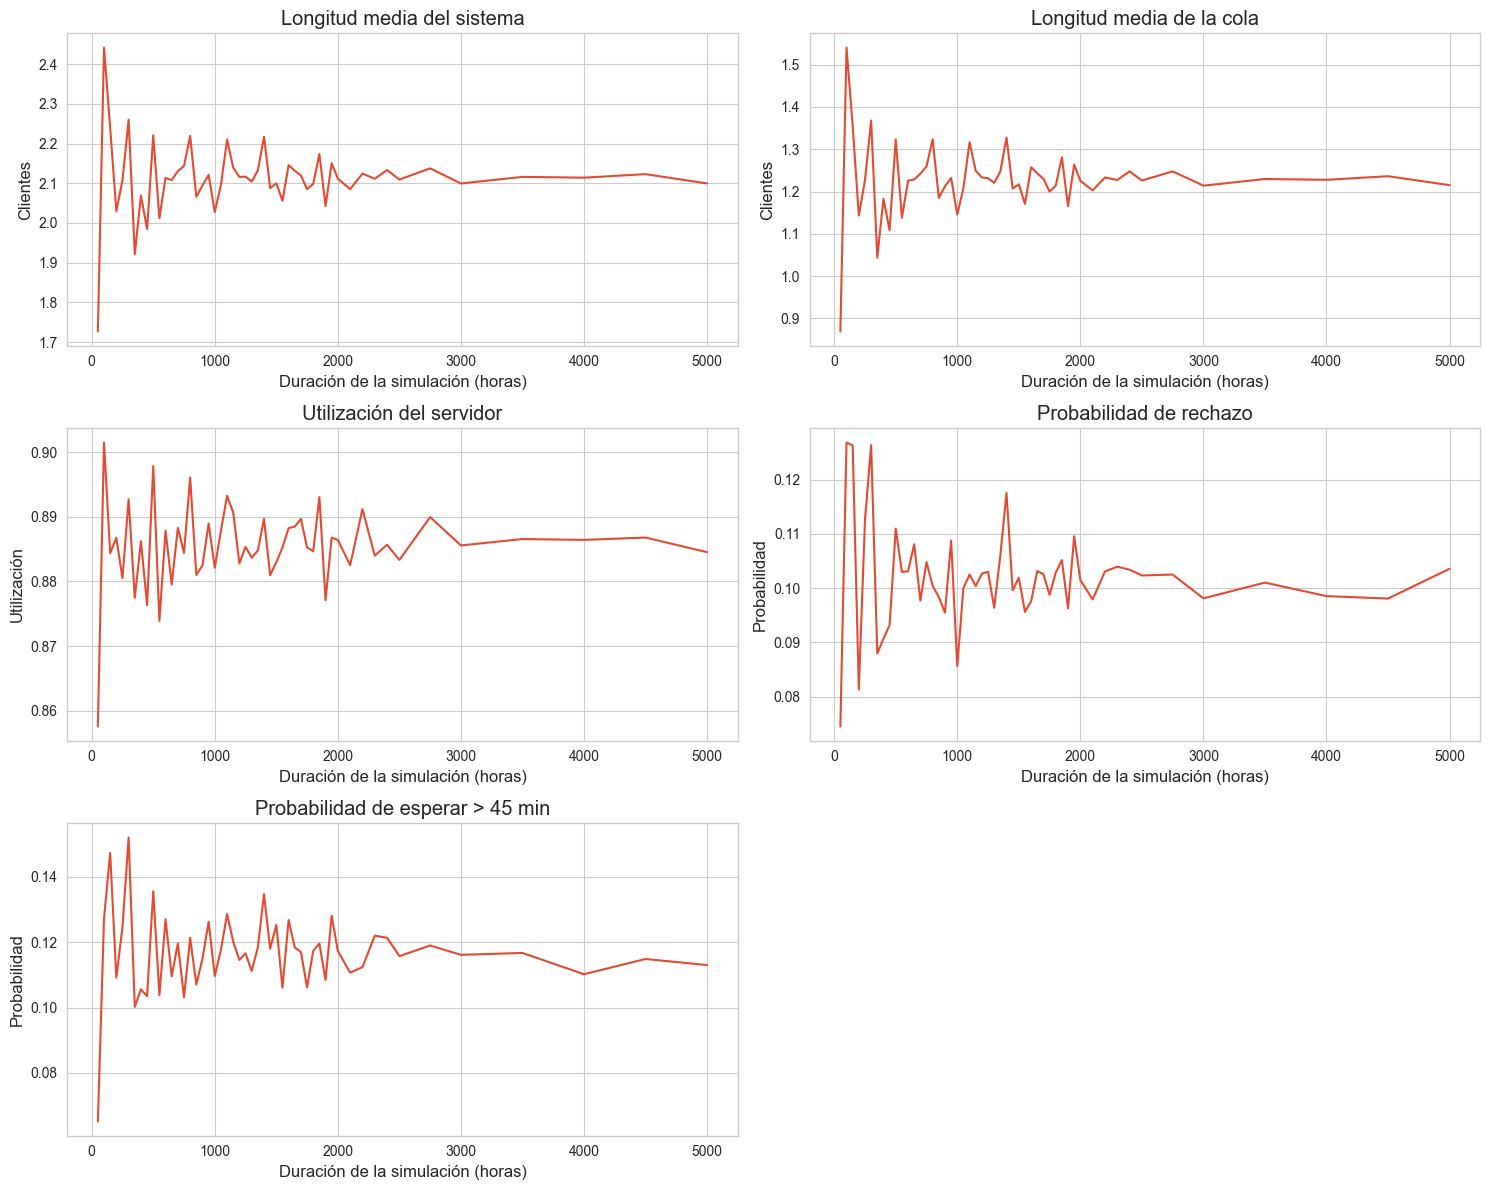
\includegraphics[width=0.8\textwidth]{convergencia_metricas.png}
    \caption{Análisis de convergencia de las diferentes métricas en función de la duración de la simulación. Se puede apreciar como se estabilizan con el paso del tiempo}
    \label{fig:convergencia}
\end{figure}

\begin{figure}[H]
    \centering
    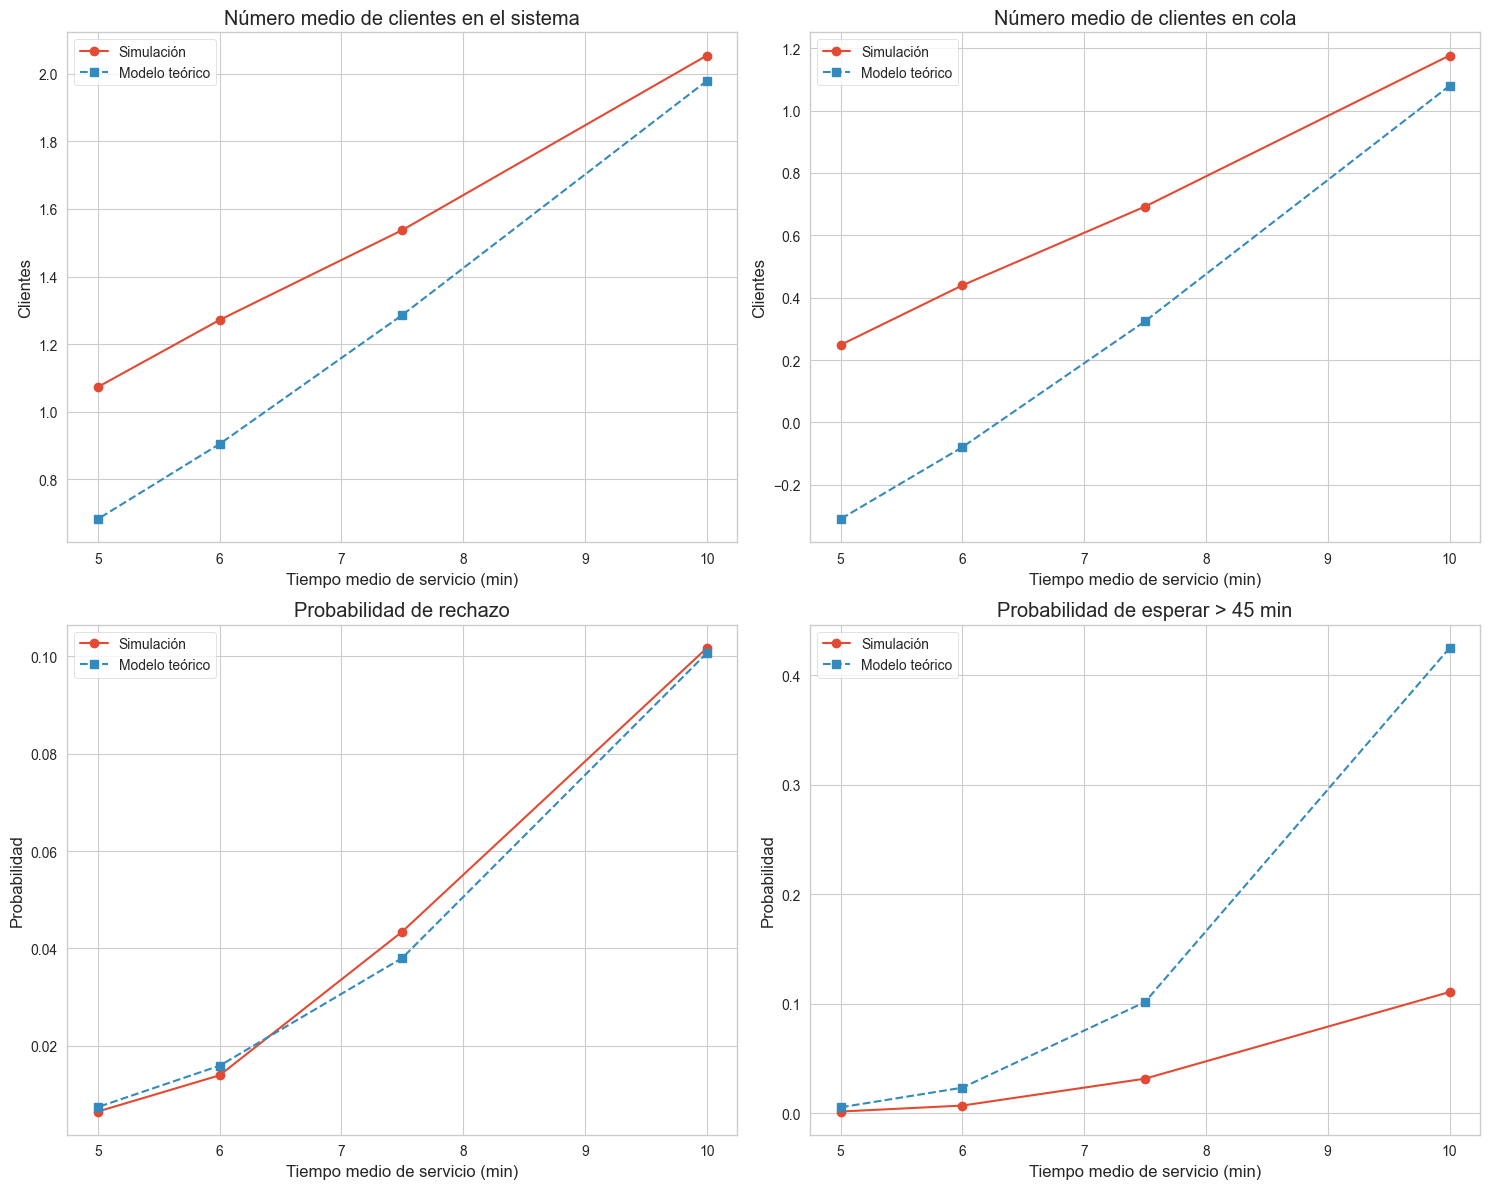
\includegraphics[width=0.8\textwidth]{analisis_sensibilidad.png}
    \caption{Análisis de sensibilidad comparando diferentes tiempos de servicio y su impacto en las métricas del sistema.}
    \label{fig:sensibilidad}
\end{figure}

\subsection{Interpretación de los resultados}

Los resultados indican que, en el escenario actual, el sistema opera cercano a su límite de capacidad, lo que genera tiempos de espera aceptables para la mayoría de los clientes, aunque con una fracción significativa de clientes que son rechazados por falta de espacio (10.6\%). 

La comparación con el modelo teórico muestra concordancia en las métricas principales, salvo algunas diferencias atribuibles a la variabilidad inherente a la simulación. La diferencia más notable se observa en la probabilidad de esperar más de 45 minutos, donde el modelo teórico predice un valor mayor (42.48\%) que el observado en la simulación (11.96\%). Esta discrepancia puede explicarse por la capacidad limitada del sistema, que "trunca" los tiempos de espera prolongados debido al mecanismo de rechazo.

El análisis de sensibilidad demuestra claramente que la reducción del tiempo de servicio (mediante la contratación de una ayudante) mejoraría significativamente el desempeño del sistema, disminuyendo tanto la probabilidad de rechazo como los tiempos de espera.

\section{Modelo Matemático}

\subsection{Descripción del modelo y supuestos}

Se utilizó el modelo M/M/1/K, donde:

\begin{itemize}
    \item \textbf{Llegadas}: Distribuidas de forma Poisson con una tasa $\lambda = 5$ clientes/hora.
    \item \textbf{Servicios}: Distribuidos exponencialmente con una tasa $\mu$ (6 clientes/hora en el escenario actual, incrementable a 12 clientes/hora en el escenario con ayudante).
    \item \textbf{Sistema}: Un único servidor con capacidad limitada a 5 clientes (1 en atención + 4 en espera).
\end{itemize}

Los supuestos clave incluyen la independencia de los tiempos interllegada y de servicio, y la atención en base al orden de llegada (FIFO).

Las fórmulas utilizadas para el modelo M/M/1/K son:

\begin{align}
\rho &= \frac{\lambda}{\mu} \\
p_0 &= \frac{1-\rho}{1-\rho^{K+1}} \\
p_k &= p_0 \cdot \rho^K \\
L &= \frac{\rho(1-(K+1)\rho^K + K\rho^{K+1})}{(1-\rho)(1-\rho^{K+1})} \\
L_q &= L - (1-p_K) \\
\lambda_{eff} &= \lambda(1-p_K) \\
W &= \frac{L}{\lambda_{eff}} \\
W_q &= \frac{L_q}{\lambda_{eff}}
\end{align}

Donde:
\begin{itemize}
    \item $\rho$ es la tasa de utilización
    \item $p_0$ es la probabilidad de sistema vacío
    \item $p_K$ es la probabilidad de sistema lleno
    \item $L$ es el número medio de clientes en el sistema
    \item $L_q$ es el número medio de clientes en cola
    \item $\lambda_{eff}$ es la tasa efectiva de llegada (excluyendo rechazos)
    \item $W$ es el tiempo medio en el sistema
    \item $W_q$ es el tiempo medio en cola
\end{itemize}

\subsection{Comparación de resultados teóricos y experimentales}

Como se observa en la sección de resultados, existe una buena correlación entre el modelo teórico y los resultados de la simulación. Las diferencias más notables se encuentran en:

\begin{itemize}
    \item La utilización del servidor: teórica 83.33\% vs. simulada 88.14\%.
    \item La probabilidad de esperar más de 45 minutos: teórica 42.48\% vs. simulada 11.96\%.
\end{itemize}

Estas diferencias se pueden atribuir a la naturaleza estocástica de la simulación y al efecto de la capacidad limitada, que en la práctica reduce la probabilidad de tiempos de espera extremadamente largos debido al mecanismo de rechazo.

\section{Conclusiones}

\begin{lstlisting}[language=bash, caption=Conclusiones de la simulación]
===== CONCLUSIONES =====
1. En el escenario actual (10 min/cliente):
   - Número medio de clientes en el salón: 2.11
   - Número medio de clientes esperando: 1.23
   - Probabilidad de no encontrar sitio: 0.1059
   - Probabilidad de esperar más de 45 min: 0.1196

2. En el escenario con ayudante (5 min/cliente):
   - Número medio de clientes en el salón: 1.07
   - Número medio de clientes esperando: 0.25
   - Probabilidad de no encontrar sitio: 0.0064
   - Probabilidad de esperar más de 45 min: 0.0013

3. Recomendación:
   Se recomienda contratar una ayudante, ya que reduciría significativamente los tiempos de espera y la probabilidad de no encontrar sitio.
\end{lstlisting}

\subsection{Resumen de hallazgos principales}

En el escenario actual (10 minutos por cliente), el sistema opera cerca de su capacidad máxima, generando tiempos de espera moderados pero con una probabilidad de rechazo considerable (alrededor del 10.6\%).

La simulación y el modelo teórico se complementan, demostrando que la dinámica del sistema se comporta de manera esperada en un ambiente de atención con recursos limitados.

El análisis de sensibilidad indica que la contratación de una ayudante, que reduce el tiempo de servicio a 5 minutos por cliente, mejora significativamente el desempeño: se reduce el número medio de clientes en el sistema (de 2.11 a 1.07) y en la cola (de 1.23 a 0.25), disminuye la probabilidad de rechazo (de 10.59\% a 0.64\%) y se acortan los tiempos de espera, con una probabilidad prácticamente nula de esperar más de 45 minutos (de 11.96\% a 0.13\%).

\subsection{Implicaciones prácticas}

Los resultados de este estudio ofrecen evidencia cuantitativa para apoyar la decisión de contratar una ayudante en la peluquería. Esta inversión en personal adicional conduciría a una mejora sustancial en la calidad del servicio, reduciendo tanto los tiempos de espera como la probabilidad de que los clientes no encuentren sitio disponible.

En conjunto, el proyecto demuestra la utilidad de la simulación de eventos discretos para analizar y optimizar sistemas de atención, y proporciona evidencia para la toma de decisiones basada en métricas cuantitativas y comparaciones con modelos teóricos.

\end{document}